\chapter{New century}

\section{Murine LTP}

Long term potentiation is MP:0002207. 255 genes are recorded with this phenotype. 140 of these are in the PSP and form an induced subgraph of 140 nodes and only 125 edges. Somewhat remarkable therefore although it has sixty components the largest has 75 elements. 1 component has three elements,four have two and 54 are singletons. 

115 were not found in the PSP. The most enriched cellular component is however synapse GO:0045202 with 51 members from a 1482 gene annotation. 

These 51 contain 4 associated with GO annotation glutamate receptor activity   (molecular function GO:008066) table~\ref{tab: Genes associated with murine long term potentiation not found in the PSP but associated with gene ontology Molecular Function GO:0008066 Glutamate receptor activity}. This is to be expected given the proteomic and interaction data driven nature of the network generation but suggests that the current network of 3457 nodes is still incomplete. Many of the genes however reflect that the PSP model is of a glutamatergic synapse. The 51 also contain other synaptic receptor components not specific to the glutamatergic synapse such as 7 listed as annotated as cellular component GABAergic synapse (table~\ref{tab:Genes associated with murine long term potentiation not found in the PSP but associated with gene ontology Cellular Component GO:0098982 GABA synapse} GO:0098982).


% latex table generated in R 3.6.2 by xtable 1.8-4 package
% Sat Feb 15 11:20:49 2020
\begin{table}[ht]
\centering
\begin{tabular}{llr}
  \hline
Gene.Symbol & Gene.Name & Entrez.Gene.ID \\ 
  \hline
NRG1 & neuregulin 1 & 3084 \\ 
  ERBB4 & erb-b2 receptor tyrosine kinase 4 & 2066 \\ 
  DRD1 & dopamine receptor D1 & 1812 \\ 
  DAG1 & dystroglycan 1 & 1605 \\ 
  LRRTM1 & leucine rich repeat transmembrane neuronal 1 & 347730 \\ 
  CNR1 & cannabinoid receptor 1 & 1268 \\ 
  GABRA5 & gamma-aminobutyric acid type A receptor subunit alpha5 & 2558 \\ 
   \hline
\end{tabular}
 \caption{Genes associated with murine long term potentiation not found in the PSP but associated with gene ontology Cellular Component GO:0098982 GABA synapse}
 \label{tab:Genes associated with murine long term potentiation not found in the PSP but associated with gene ontology Cellular Component GO:0098982 GABA synapse}
\end{table}



% latex table generated in R 3.6.2 by xtable 1.8-4 package
% Sat Feb 15 11:07:14 2020
\begin{table}[ht]
\centering
\begin{tabular}{rllr}
  \hline
 & Gene Symbol & Gene Name & Entrez ID \\ 
  \hline
1 & CNIH2 & cornichon family AMPA receptor auxiliary protein 2 & 254263 \\ 
  2 & SHISA7 &  shisa family member 7 & 729956 \\ 
  3 & CNIH3 & cornichon family AMPA receptor auxiliary protein 3 & 149111 \\ 
  4 & OPRM1 & opioid receptor mu 1) & 4988 \\ 
   \hline
\end{tabular}
\caption{Genes associated with murine long term potentiation not found in the PSP but associated with gene ontology Molecular Function GO:0008066 Glutamate receptor activity}
\label{tab: Genes associated with murine long term potentiation not found in the PSP but associated with gene ontology Molecular Function GO:0008066 Glutamate receptor activity}
\end{table}



\subsection{Giant connected component}

The giant component within the murine LTP subgraph has 75 nodes and 119 edges (which seems very efficient just over ratio for condition of giant component). This giant component spans 19 communities but the most numerous are group 20 and group 5 (n=13, 17.33\%, n=9 12.0\%).

Groups 5 and 20 are the two statistically significantly over-represented after correction for multiple comparisons (Module 20 p-value = 0.0001 , OR= 3.97, 95 percent confidence interval:1.973 7.403) and Module 5
p-value = 0.001615, OR=3.702 95 percent confidence interval:1.589 7.661) , Fisher's exact test alpha bonferroni = 0.0026\footnote{all code \url{source('~/RProjects/centrality/R/mouse_ltp.R')}} see table~\ref{tab:Distribution of genes association with murine long term potentiation over community modules detected using spectral clustering}.

\subsubsection{Degree in giant connected component}
The mean 


% latex table generated in R 3.6.2 by xtable 1.8-4 package
% Sat Feb 15 12:29:02 2020
% source('~/RProjects/centrality/R/mouse_ltp.R')
\begin{table}[ht]
\centering
\begin{tabular}{lccrr}
  \hline
Module & Number in Subgraph & Number in PSP & OR & p \\ 
  \hline
20 & 13 & 151 & 3.966 & 0.00011 \\ 
  5 &  9 & 112 & 3.702 & 0.00162 \\ 
  33 &  7 & 191 & 1.689 & 0.20464 \\ 
  26 &  7 & 120 & 2.688 & 0.02255 \\ 
  7 &  7 & 129 & 2.500 & 0.03102 \\ 
  16 &  6 & 72 & 3.838 & 0.00751 \\ 
  17 &  4 & 148 & 1.246 & 0.56712 \\ 
  9 &  4 & 65 & 2.835 & 0.06344 \\ 
  24 &  3 & 76 & 1.819 & 0.24267 \\ 
  44 &  2 & 103 & 0.895 & 1.00000 \\ 
  22 &  2 & 42 & 2.194 & 0.24451 \\ 
  10 &  2 & 154 & 0.599 & 0.77178 \\ 
  2 &  2 & 165 & 0.559 & 0.58261 \\ 
  1 &  2 & 171 & 0.539 & 0.58370 \\ 
  51 &  1 & 112 & 0.412 & 0.73137 \\ 
  43 &  1 & 150 & 0.307 & 0.37301 \\ 
  28 &  1 & 38 & 1.213 & 0.56981 \\ 
  11 &  1 & 56 & 0.823 & 1.00000 \\ 
  3 &  1 & 41 & 1.124 & 0.59668 \\ 
   \hline
 
\end{tabular}
\caption{Distribution of genes association with murine long term potentiation over community modules detected using spectral clustering. $\alpha$ bonferroni=0.0026, Fisher's exact test}
\label{tab:Distribution of genes association with murine long term potentiation over community modules detected using spectral clustering}
\end{table}


\begin{figure}
    \centering
    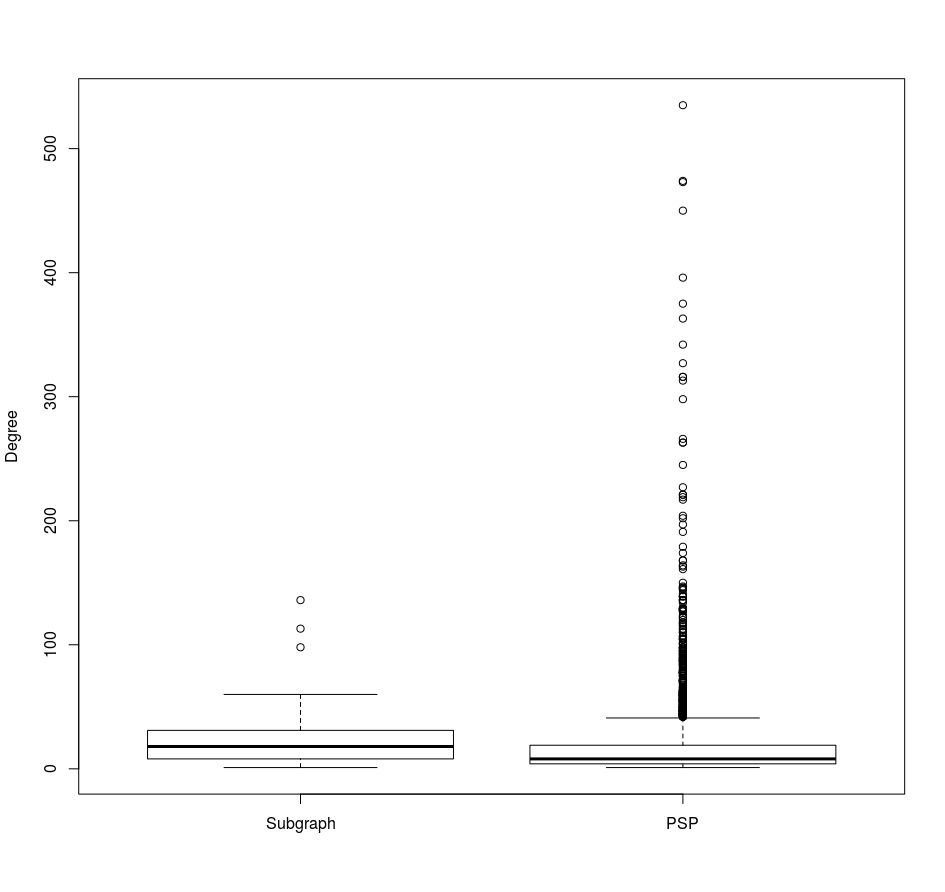
\includegraphics[width=\textwidth]{images/Rplot_boxplot_subgraph_and_PSP_degree.png}
    \caption{Degree distribution for induced subgraph of murine long term potentiation genes compared with PSP. The largest hub not has been removed from the subgraph.}
    \label{fig:Degree distribution for induced subgraph of murine long term potentiation genes compared with PSP. The largest hub not has been removed from the subgraph}
\end{figure}







\includegraphics[height=\baselineskip]{example-image}.
\begin{figure}
\includegraphics[height=3cm]{example-image-a}\includegraphics[width=5cm]{example-image-b}

\includegraphics[height=3cm]{example-image-a} \includegraphics[width=5cm]{example-image-b}
\caption{A figure}

\end{figure}
